\PassOptionsToPackage{unicode=true}{hyperref} % options for packages loaded elsewhere
\PassOptionsToPackage{hyphens}{url}
%
\documentclass[]{article}
\usepackage{lmodern}
\usepackage{amssymb,amsmath}
\usepackage{ifxetex,ifluatex}
\usepackage{fixltx2e} % provides \textsubscript
\ifnum 0\ifxetex 1\fi\ifluatex 1\fi=0 % if pdftex
  \usepackage[T1]{fontenc}
  \usepackage[utf8]{inputenc}
  \usepackage{textcomp} % provides euro and other symbols
\else % if luatex or xelatex
  \usepackage{unicode-math}
  \defaultfontfeatures{Ligatures=TeX,Scale=MatchLowercase}
\fi
% use upquote if available, for straight quotes in verbatim environments
\IfFileExists{upquote.sty}{\usepackage{upquote}}{}
% use microtype if available
\IfFileExists{microtype.sty}{%
\usepackage[]{microtype}
\UseMicrotypeSet[protrusion]{basicmath} % disable protrusion for tt fonts
}{}
\IfFileExists{parskip.sty}{%
\usepackage{parskip}
}{% else
\setlength{\parindent}{0pt}
\setlength{\parskip}{6pt plus 2pt minus 1pt}
}
\usepackage{hyperref}
\hypersetup{
            pdftitle={Bayesian Artillery},
            pdfauthor={Alberto Dell'Era},
            pdfborder={0 0 0},
            breaklinks=true}
\urlstyle{same}  % don't use monospace font for urls
\usepackage[margin=1in]{geometry}
\usepackage{color}
\usepackage{fancyvrb}
\newcommand{\VerbBar}{|}
\newcommand{\VERB}{\Verb[commandchars=\\\{\}]}
\DefineVerbatimEnvironment{Highlighting}{Verbatim}{commandchars=\\\{\}}
% Add ',fontsize=\small' for more characters per line
\usepackage{framed}
\definecolor{shadecolor}{RGB}{248,248,248}
\newenvironment{Shaded}{\begin{snugshade}}{\end{snugshade}}
\newcommand{\AlertTok}[1]{\textcolor[rgb]{0.94,0.16,0.16}{#1}}
\newcommand{\AnnotationTok}[1]{\textcolor[rgb]{0.56,0.35,0.01}{\textbf{\textit{#1}}}}
\newcommand{\AttributeTok}[1]{\textcolor[rgb]{0.77,0.63,0.00}{#1}}
\newcommand{\BaseNTok}[1]{\textcolor[rgb]{0.00,0.00,0.81}{#1}}
\newcommand{\BuiltInTok}[1]{#1}
\newcommand{\CharTok}[1]{\textcolor[rgb]{0.31,0.60,0.02}{#1}}
\newcommand{\CommentTok}[1]{\textcolor[rgb]{0.56,0.35,0.01}{\textit{#1}}}
\newcommand{\CommentVarTok}[1]{\textcolor[rgb]{0.56,0.35,0.01}{\textbf{\textit{#1}}}}
\newcommand{\ConstantTok}[1]{\textcolor[rgb]{0.00,0.00,0.00}{#1}}
\newcommand{\ControlFlowTok}[1]{\textcolor[rgb]{0.13,0.29,0.53}{\textbf{#1}}}
\newcommand{\DataTypeTok}[1]{\textcolor[rgb]{0.13,0.29,0.53}{#1}}
\newcommand{\DecValTok}[1]{\textcolor[rgb]{0.00,0.00,0.81}{#1}}
\newcommand{\DocumentationTok}[1]{\textcolor[rgb]{0.56,0.35,0.01}{\textbf{\textit{#1}}}}
\newcommand{\ErrorTok}[1]{\textcolor[rgb]{0.64,0.00,0.00}{\textbf{#1}}}
\newcommand{\ExtensionTok}[1]{#1}
\newcommand{\FloatTok}[1]{\textcolor[rgb]{0.00,0.00,0.81}{#1}}
\newcommand{\FunctionTok}[1]{\textcolor[rgb]{0.00,0.00,0.00}{#1}}
\newcommand{\ImportTok}[1]{#1}
\newcommand{\InformationTok}[1]{\textcolor[rgb]{0.56,0.35,0.01}{\textbf{\textit{#1}}}}
\newcommand{\KeywordTok}[1]{\textcolor[rgb]{0.13,0.29,0.53}{\textbf{#1}}}
\newcommand{\NormalTok}[1]{#1}
\newcommand{\OperatorTok}[1]{\textcolor[rgb]{0.81,0.36,0.00}{\textbf{#1}}}
\newcommand{\OtherTok}[1]{\textcolor[rgb]{0.56,0.35,0.01}{#1}}
\newcommand{\PreprocessorTok}[1]{\textcolor[rgb]{0.56,0.35,0.01}{\textit{#1}}}
\newcommand{\RegionMarkerTok}[1]{#1}
\newcommand{\SpecialCharTok}[1]{\textcolor[rgb]{0.00,0.00,0.00}{#1}}
\newcommand{\SpecialStringTok}[1]{\textcolor[rgb]{0.31,0.60,0.02}{#1}}
\newcommand{\StringTok}[1]{\textcolor[rgb]{0.31,0.60,0.02}{#1}}
\newcommand{\VariableTok}[1]{\textcolor[rgb]{0.00,0.00,0.00}{#1}}
\newcommand{\VerbatimStringTok}[1]{\textcolor[rgb]{0.31,0.60,0.02}{#1}}
\newcommand{\WarningTok}[1]{\textcolor[rgb]{0.56,0.35,0.01}{\textbf{\textit{#1}}}}
\usepackage{longtable,booktabs}
% Fix footnotes in tables (requires footnote package)
\IfFileExists{footnote.sty}{\usepackage{footnote}\makesavenoteenv{longtable}}{}
\usepackage{graphicx,grffile}
\makeatletter
\def\maxwidth{\ifdim\Gin@nat@width>\linewidth\linewidth\else\Gin@nat@width\fi}
\def\maxheight{\ifdim\Gin@nat@height>\textheight\textheight\else\Gin@nat@height\fi}
\makeatother
% Scale images if necessary, so that they will not overflow the page
% margins by default, and it is still possible to overwrite the defaults
% using explicit options in \includegraphics[width, height, ...]{}
\setkeys{Gin}{width=\maxwidth,height=\maxheight,keepaspectratio}
\setlength{\emergencystretch}{3em}  % prevent overfull lines
\providecommand{\tightlist}{%
  \setlength{\itemsep}{0pt}\setlength{\parskip}{0pt}}
\setcounter{secnumdepth}{0}
% Redefines (sub)paragraphs to behave more like sections
\ifx\paragraph\undefined\else
\let\oldparagraph\paragraph
\renewcommand{\paragraph}[1]{\oldparagraph{#1}\mbox{}}
\fi
\ifx\subparagraph\undefined\else
\let\oldsubparagraph\subparagraph
\renewcommand{\subparagraph}[1]{\oldsubparagraph{#1}\mbox{}}
\fi

% set default figure placement to htbp
\makeatletter
\def\fps@figure{htbp}
\makeatother


\title{Bayesian Artillery}
\author{Alberto Dell'Era}
\date{}

\begin{document}
\maketitle

\emph{A short summary is available at:\\
\url{https://github.com/alberto-dellera/bayesian_artillery/blob/master/README.md}
}~\\
\emph{Github readers: github on-line resolution is very low, I'd suggest
to download this pdf and open it}

A battery is shooting at us, and all we have are some noisy radar
readings about the projectile trajectory:

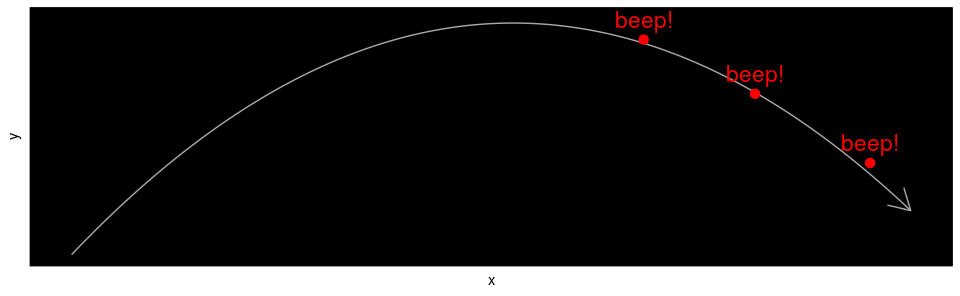
\includegraphics{static_images/simulate_cartoon-1.png}

we want to find the battery position, also factoring in some prior
knowledge provided by our Intelligence.

\hypertarget{summary}{%
\subsubsection{Summary}\label{summary}}

We will perform a standard Bayesian analysis (model building, MCMC by
JAGS, chains exploration, etc), but from the practical perspective of
the physical (mechanical) domain expert that wants to understand how the
algorithm ``reasons'' about trajectories, projectile speed, etc etc.

In particular, we will explore how the Bayesian system incrementally
improves its estimation as soon as a new radar reading enters the
system.

I will often reference the marvellous\footnote{a joy to read - and with
  all five-stars reviews on Amazon, if you consider that almost all
  reviews with less then five-stars blame the Kindle formatting (that
  has issues with formulae), not the content at all} book ``Doing
Bayesian Data Analysis'' (Kruschke
\protect\hyperlink{ref-DBDA2E}{2015}), where most of my Bayesian
knowledge comes from.

\hypertarget{motivation}{%
\subsubsection{Motivation}\label{motivation}}

\begin{itemize}
\tightlist
\item
  to practice Bayesian analysis in a concrete and well-known setting
\item
  to get a first impression of how it looks like to extend classic
  models (Physical, Electrical, Financial, etc) to incorporate domain
  (prior) knowledge
\item
  for statistical fun
\item
  for programming fun
\end{itemize}

not necessarily in order of importance.

\hypertarget{physical-model}{%
\section{Physical model}\label{physical-model}}

The physical model is composed by a \emph{deterministic} part (the
trajectory) and a \emph{statistical} one (the error characterization),
that together describe the radar readings that we osberve:

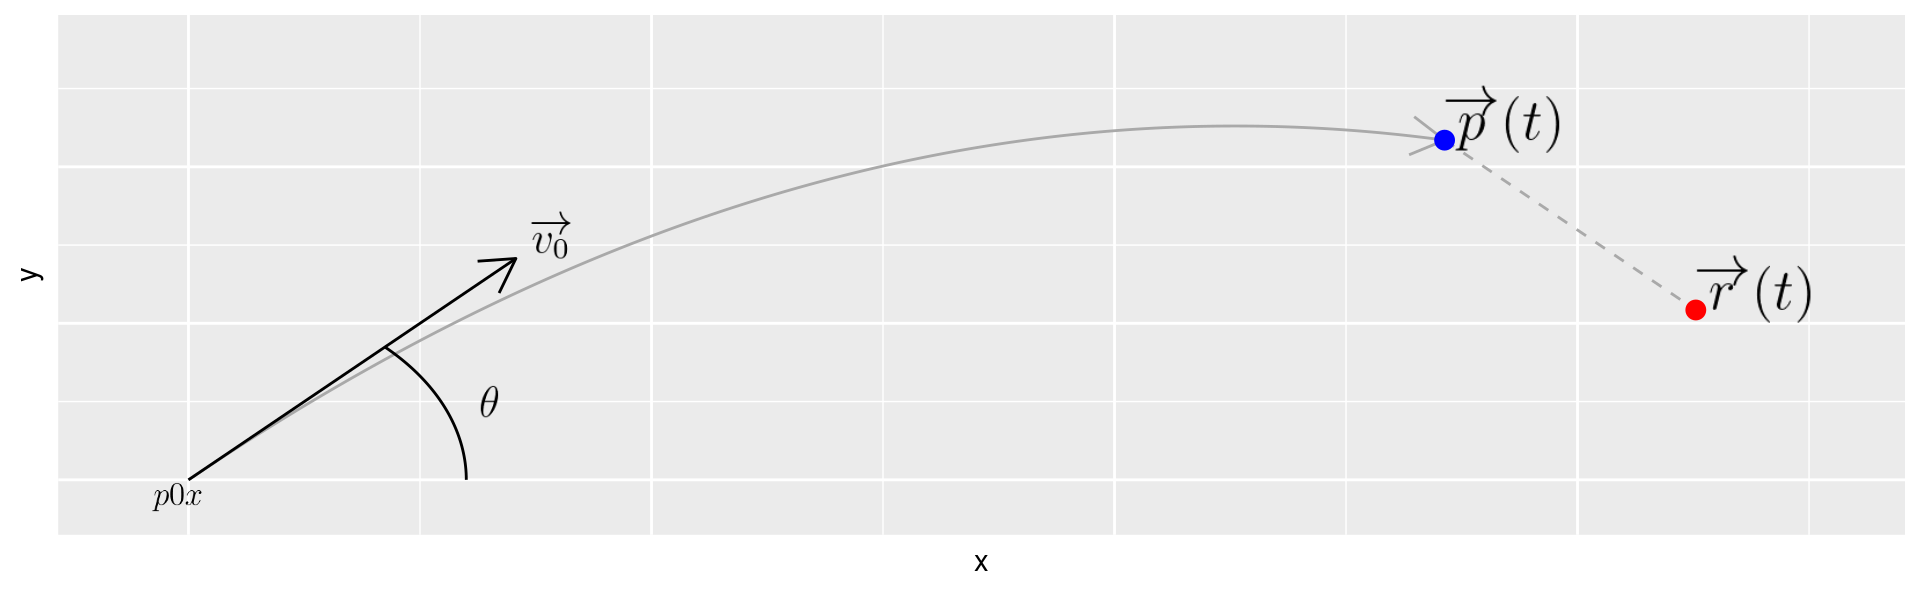
\includegraphics{static_images/physical_model_figure-1.png}

The trajectory is described by the position vector
\(\overrightarrow{p}(t)\), that must satisfy the usual differential
equation \(\ddot{\overrightarrow{p}}(t)=\overrightarrow{g}\), where
\(\overrightarrow{g}\) is the gravitational acceleration. It is
well-known that \(\overrightarrow{p}(t)\) is perfectly and
deterministically dictated by the initial state of the system (position
and velocity when the battery fired at time \(t_0\)), i.e.~by this
quartet of four parameters:

\begin{itemize}
\tightlist
\item
  \(p_{0x}\), the sought-after position of the battery, i.e.
  \(\overrightarrow{p}(t_o)_x\)
\item
  \(v_0\), the modulus of the initial velocity \(\overrightarrow{v_0}\),
  aka ``muzzle velocity''
\item
  \(\theta\), the barrel elevation angle
\item
  \(t_0\), the time when the battery fired.
\end{itemize}

The radar readings are simply
\(\overrightarrow{r}(t_i)=\overrightarrow{p}(t_i)+\overrightarrow{e}(t_i)\),
that is, the trajectory sampled by the radar at some instants \(t_i\)
plus some reading error \(\overrightarrow{e}\) (aka ``measurement
error'').

The radar was built by our military-industrial complex, and hence we
know everything about it: our ACME-MARK3 radar samples the sky using a
constant sampling period (picture a quickly rotating radar as seen in
movies\ldots{}) and we know the stochastic characteristics of its error
\(\overrightarrow{e}\). To keep things simple\footnote{in a real
  setting, we should observe that (for a classic rotating radar) the
  distance is estimated by the time the radiowave takes to bounch off
  the projectile, and the direction by the location of the intensity
  peek of the received radio echo during the radar rotation. Both are
  two very different physical processes (the former electrical, the
  latter mechanical), maybe approximately Gaussian, maybe indipendent,
  but with different standard deviations for sure; we should therefore
  at least vary the covariance matrix depending on the polar coordinates
  of the trajectory with respect to the radar location. Very fun, but I
  want to focus on the Bayesian part, not on the model adherence to
  reality.}, we will make the usual toy assumptions that
\(\overrightarrow{e}\) samples are i.i.e. (Indipendent and Identically
Distributed) as a normal distribution, with mean zero (otherwise it
would not be an error) and perfectly known covariance matrix, with
indipendent components \(\overrightarrow{e}_x\) and
\(\overrightarrow{e}_y\) both sharing the same value \(\sigma_e\) of the
standard deviation\footnote{i.e.~the covariance matrix is
  \[\Sigma = \begin{bmatrix} \sigma_e^2 & 0 \\
  0 & \sigma_e^2  \\
  \end{bmatrix} \]}.

We have enough information to simulate the stochastic process:

\begin{Shaded}
\begin{Highlighting}[]
\NormalTok{simulate <-}\StringTok{ }\ControlFlowTok{function}\NormalTok{(n,        }\CommentTok{# number of readings }
\NormalTok{                     t0,       }\CommentTok{# sec}
\NormalTok{                     p0x,      }\CommentTok{# m}
\NormalTok{                     v0,       }\CommentTok{# m/s}
\NormalTok{                     theta,    }\CommentTok{# rad}
\NormalTok{                     error.sd, }\CommentTok{# m}
                     \DataTypeTok{time.interval =} \KeywordTok{c}\NormalTok{(}\DecValTok{0}\NormalTok{, }\DecValTok{1}\NormalTok{) }\CommentTok{# as fraction of flight time}
\NormalTok{                    ) }
\NormalTok{\{}
\NormalTok{  v0x <-}\StringTok{ }\NormalTok{v0 }\OperatorTok{*}\StringTok{ }\KeywordTok{cos}\NormalTok{(theta)  }
\NormalTok{  v0y <-}\StringTok{ }\NormalTok{v0 }\OperatorTok{*}\StringTok{ }\KeywordTok{sin}\NormalTok{(theta)}
  
  \CommentTok{# calculate final impact figures }
\NormalTok{  flight_time <-}\StringTok{ }\DecValTok{2} \OperatorTok{*}\StringTok{ }\NormalTok{v0y }\OperatorTok{/}\StringTok{ }\NormalTok{g}
\NormalTok{  tf  <-}\StringTok{ }\NormalTok{t0 }\OperatorTok{+}\StringTok{ }\NormalTok{flight_time}
\NormalTok{  pfx <-}\StringTok{ }\NormalTok{p0x }\OperatorTok{+}\StringTok{ }\NormalTok{v0x }\OperatorTok{*}\StringTok{ }\NormalTok{flight_time}
  
  \CommentTok{# sample time at uniform intervals}
\NormalTok{  t <-}\StringTok{ }\KeywordTok{seq}\NormalTok{(t0 }\OperatorTok{+}\StringTok{ }\NormalTok{time.interval[[}\DecValTok{1}\NormalTok{]]}\OperatorTok{*}\NormalTok{flight_time, }
\NormalTok{           t0 }\OperatorTok{+}\StringTok{ }\NormalTok{time.interval[[}\DecValTok{2}\NormalTok{]]}\OperatorTok{*}\NormalTok{flight_time, }
           \DataTypeTok{length.out =}\NormalTok{ n)}

  \CommentTok{# sample trajectory}
\NormalTok{  px <-}\StringTok{ }\NormalTok{p0x }\OperatorTok{+}\StringTok{ }\NormalTok{v0x }\OperatorTok{*}\StringTok{ }\NormalTok{(t }\OperatorTok{-}\StringTok{ }\NormalTok{t0)}
\NormalTok{  py <-}\StringTok{   }\DecValTok{0} \OperatorTok{+}\StringTok{ }\NormalTok{v0y }\OperatorTok{*}\StringTok{ }\NormalTok{(t }\OperatorTok{-}\StringTok{ }\NormalTok{t0) }\OperatorTok{-}\StringTok{ }\FloatTok{0.5} \OperatorTok{*}\StringTok{ }\NormalTok{g }\OperatorTok{*}\StringTok{ }\NormalTok{(t }\OperatorTok{-}\StringTok{ }\NormalTok{t0)}\OperatorTok{^}\DecValTok{2}
  
  \CommentTok{# add radar error }
\NormalTok{  rx <-}\StringTok{ }\NormalTok{px }\OperatorTok{+}\StringTok{ }\KeywordTok{rnorm}\NormalTok{(n, }\DecValTok{0}\NormalTok{, error.sd)}
\NormalTok{  ry <-}\StringTok{ }\NormalTok{py }\OperatorTok{+}\StringTok{ }\KeywordTok{rnorm}\NormalTok{(n, }\DecValTok{0}\NormalTok{, error.sd)}
  
  \KeywordTok{tibble}\NormalTok{(}\DataTypeTok{i=}\DecValTok{1}\OperatorTok{:}\NormalTok{n, }\DataTypeTok{t=}\NormalTok{t, }\DataTypeTok{rx=}\NormalTok{rx, }\DataTypeTok{ry=}\NormalTok{ry)}
\NormalTok{\}}
\end{Highlighting}
\end{Shaded}

And we observe this single shot of the battery, that we will use from
now on as the input to our algorithm:

\begin{Shaded}
\begin{Highlighting}[]
\CommentTok{# radar readings (samples of trajectory, plus reading error)}
\KeywordTok{set.seed}\NormalTok{(}\DecValTok{4321}\NormalTok{)}
\NormalTok{readings <-}\StringTok{ }\KeywordTok{simulate}\NormalTok{(readings.n, }
                     \DataTypeTok{t0=}\DecValTok{0}\NormalTok{, }\DataTypeTok{p0x=}\NormalTok{p0x.true, }\DataTypeTok{v0=}\NormalTok{v0.true, }\DataTypeTok{theta=}\NormalTok{theta.true, }
                     \DataTypeTok{error.sd=}\NormalTok{readings.error.sd,}
                     \DataTypeTok{time.interval =} \KeywordTok{c}\NormalTok{(}\FloatTok{0.65}\NormalTok{, }\FloatTok{0.9}\NormalTok{))  }

\CommentTok{# true trajectory}
\NormalTok{trajectory <-}\StringTok{ }\KeywordTok{simulate}\NormalTok{(}\DecValTok{300}\NormalTok{, }
                       \DataTypeTok{t0=}\DecValTok{0}\NormalTok{, }\DataTypeTok{p0x=}\NormalTok{p0x.true, }\DataTypeTok{v0=}\NormalTok{v0.true, }\DataTypeTok{theta=}\NormalTok{theta.true, }
                       \DataTypeTok{error.sd=}\DecValTok{0}\NormalTok{,}
                       \DataTypeTok{time.interval =} \KeywordTok{c}\NormalTok{(}\DecValTok{0}\NormalTok{, }\FloatTok{0.95}\NormalTok{))}

\KeywordTok{ggplot}\NormalTok{() }\OperatorTok{+}\StringTok{ }
\StringTok{  }\KeywordTok{geom_line}\NormalTok{(}\DataTypeTok{data=}\NormalTok{trajectory, }\KeywordTok{aes}\NormalTok{(}\DataTypeTok{x=}\NormalTok{rx,}\DataTypeTok{y=}\NormalTok{ry), }\DataTypeTok{arrow=}\NormalTok{grid}\OperatorTok{::}\KeywordTok{arrow}\NormalTok{(), }\DataTypeTok{color=}\StringTok{"darkgray"}\NormalTok{) }\OperatorTok{+}
\StringTok{  }\KeywordTok{geom_point}\NormalTok{(}\DataTypeTok{data=}\NormalTok{readings, }\KeywordTok{aes}\NormalTok{(}\DataTypeTok{x=}\NormalTok{rx, }\DataTypeTok{y=}\NormalTok{ry), }\DataTypeTok{color=}\StringTok{"red"}\NormalTok{) }\OperatorTok{+}
\StringTok{  }\KeywordTok{xlab}\NormalTok{(}\StringTok{"x [m]"}\NormalTok{) }\OperatorTok{+}\StringTok{ }\KeywordTok{ylab}\NormalTok{(}\StringTok{"y [m]"}\NormalTok{)}
\end{Highlighting}
\end{Shaded}

\begin{center}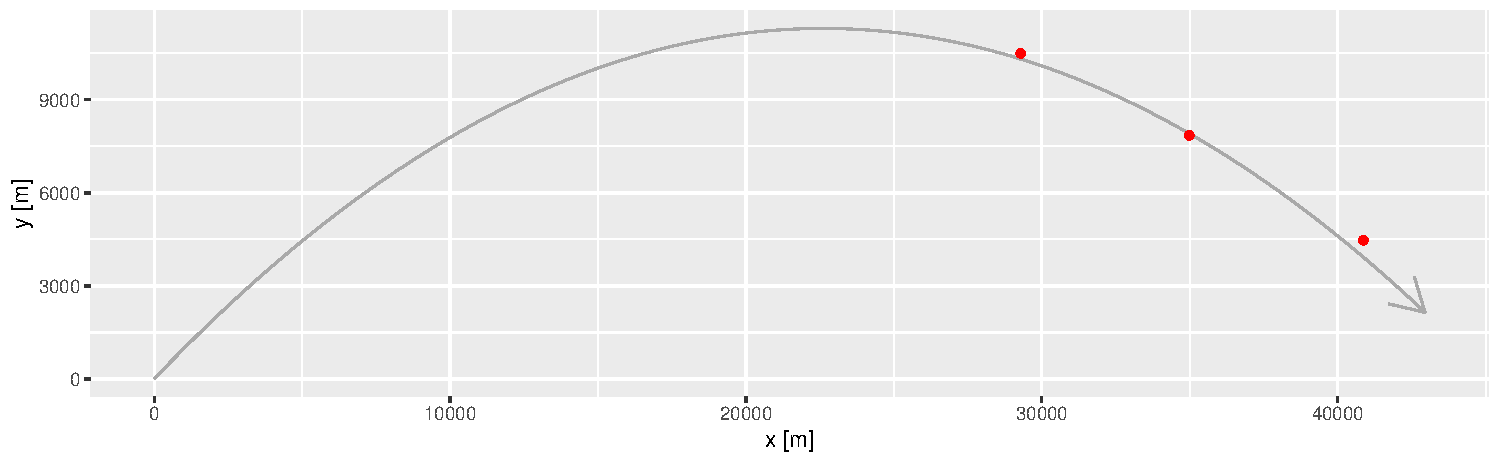
\includegraphics[width=1.0\textwidth]{bayesian_artillery_files/figure-latex/simulate-1} \end{center}

\begin{longtable}[]{@{}rrrr@{}}
\toprule
i & t & rx & ry\tabularnewline
\midrule
\endhead
1 & 62.40704 & 29282.85 & 10496.701\tabularnewline
2 & 74.40839 & 34985.47 & 7852.220\tabularnewline
3 & 86.40975 & 40872.61 & 4471.658\tabularnewline
\bottomrule
\end{longtable}

We can use a mere three readings at the end of the trajectory because
our radar, located near the battery's target, can observe just a narrow
region of the sky next to it.

\hypertarget{bayesian-model}{%
\section{Bayesian model}\label{bayesian-model}}

Here is the JAGS Bayesian model (illustrated below):

\begin{Shaded}
\begin{Highlighting}[]
\NormalTok{jagsModel <-}\StringTok{ "}
\StringTok{model \{}
\StringTok{  for ( i in 1:N ) \{}
\StringTok{    ## radar readings (likelihood)}
\StringTok{    rx[i] ~ dnorm( px[i], 1/readings.error.sd^2 )}
\StringTok{    ry[i] ~ dnorm( py[i], 1/readings.error.sd^2 )}
\StringTok{    }
\StringTok{    ## positions }
\StringTok{    px[i] <- p0x + v0x * (t[i] - t0)}
\StringTok{    py[i] <-   0 + v0y * (t[i] - t0) - 0.5 * g * (t[i] - t0)^2}
\StringTok{  \}}
\StringTok{  }
\StringTok{  ## v0 components}
\StringTok{  v0x <- v0 * cos(theta)}
\StringTok{  v0y <- v0 * sin(theta)}
\StringTok{    }
\StringTok{  # priors   }
\StringTok{  p0x   ~ dnorm( priorP0xMean, 1/priorP0xSd^2 ) # see discussion}
\StringTok{  v0    ~ dunif( 1 * 343, 3 * 343 )  # between MACH1 and MACH3}
\StringTok{  theta ~ dunif( 0, pi/2 )           # aiming above ground and not backwards}
\StringTok{  t0    ~ dunif( t[1] - 1000, t[1] ) # at most 1000 seconds before first radar reading time}
\StringTok{\}}
\StringTok{"} 
\end{Highlighting}
\end{Shaded}

The physical model already implicitly specified the Likelihood, that is,
the probability of observing the data (the three
\(\overrightarrow{r}(t_i)\) and their corresponding \(t_i\)) given the
four parameters. The formula\footnote{\(\Pr( D \mid p_{0x}, v_0, \theta, t_0 ) = \prod_{i=1}^{3} \mathcal{f_N}(\overrightarrow{r}(t_i) - \overrightarrow{p}(t_i),\,\Sigma)\);
  \(\Sigma\) as before; actually a density, not a probability} is simple
and can be easily reverse-engineered from the JAGS model text; I like to
note that it can be mentally constructed by ``plugging the four
numbers'' into the battery, firing the projectile and then following
(simulating\footnote{we can actually \emph{calculate} the trajectory
  since we were able to obtain the trajectory as a closed form solution.
  If we were to use a more realistic physical model (that e.g.~considers
  also the air friction, the different air density at various altitudes
  etc) we would need to turn to \emph{numerical simulation}, following
  the projectile using a program.}) the projectile as it travels across
the sky, writing down its positions at the three \(t_i\) instants,
substracting the actual readings, calculating the three values of the
Gaussian PDFs, and eventually multiplying.

Please also note that the JAGS model is essentially a
\emph{copy-and-paste of the physical model simulator above}, plus the
priors. That's the beauty of the Bayesian approach that Laplace has
given us: we just need to reason about how to generate (describe) the
data given the parameters (which is relatively easy), and then have the
computer turn it around from the data to the parameters\footnote{that's
  the reason why the Bayesian approach is also known as ``inverse
  probability''}.

Side note: ince almost all classical Physical models (in Mechanics,
Thermodinamics, Electrical Engineering, etc etc) are composed by a
deterministic part (like our trajectory) plus a measurement error
(usually Gaussian) that produces the data (like our radar readings),
from which the Likelihood functions is readily obtained, that means that
we can leverage the sophisticated models produced by hundreds of years
of scientific/engineering results and rather easily extend them to
incorporate any other knowledge about the parameters (the priors). Isn't
this great?

\hypertarget{choice-of-priors}{%
\subsection{choice of priors}\label{choice-of-priors}}

We will choose all mildly informative priors, obviously with the
exception of the battery position.

\hypertarget{battery-position-p_0x}{%
\subsubsection{\texorpdfstring{battery position
\(p_{0x}\)}{battery position p\_\{0x\}}}\label{battery-position-p_0x}}

Our Intelligence Department has sent us a note:

``The battery is located at x=100 meters, plus/minus 800 meters.''

Turning this statement into a mathematical expression is one of the
hardest part in Bayesian analysis, and depends on how much the
Intelligence Department is credible (Are they trustable? Are they
precise or sloppy? Have they provided good estimates in the past?) and
on their culture and language as well (What they mean by
``plus/minus''?). And this choice is critical, since a wrongly
informative prior can badly influence the posterior, and a
well-constructed one, at the opposite, can greatly enhance our chances
of success. We hence performed a thorought investigation and assesment
about the statement.

We will compare two possible outcomes:

\begin{itemize}
\tightlist
\item
  ``Intelligent Intelligence'': they are smart and cautious, their
  plus/minus represents their uncertainty well, and they do not exclude
  that the battery is outside that range. We will hence model the prior
  as a Gaussian with mean 100m and standard deviation 800m;
\item
  ``Uninformative'': their estimate is junk, we are better off ignoring
  them. A good uninformative prior would be an uniform distribution
  covering the whole battlefield; but for simplicity we will use a
  Gaussian with a gigantic standard deviation (to keep the JAGS model
  code simple; I have experimented with an uniform as well and the
  results are qualitatively the same).
\end{itemize}

Spoiler: the true battery position is at x=0; the first choice would be
the best.

\hypertarget{initial-velocity-v_0}{%
\subsubsection{\texorpdfstring{initial velocity
\(v_0\)}{initial velocity v\_0}}\label{initial-velocity-v_0}}

We don't know the battery model, and hence we will assume the typical
range of a common howitzer: between MACH1\footnote{speed of sound of air
  near the battery location; assumed as 343 m/s (normal conditions: sea
  level, 20°C, etc)} and MACH3. We have no preference for any velocity,
and hence we will use an uniform distribution.

\hypertarget{barrel-elevation-theta}{%
\subsubsection{\texorpdfstring{barrel elevation
\(\theta\)}{barrel elevation \textbackslash{}theta}}\label{barrel-elevation-theta}}

No preference either for the elevation; we will assume a uniform
distribution between 0 and \(\pi/2\) rad (that is, the battery does not
aim underground and aims to the right).

\hypertarget{firing-time-t_0}{%
\subsubsection{\texorpdfstring{firing time
\(t_0\)}{firing time t\_0}}\label{firing-time-t_0}}

We will very conservatively assume that the battery fired at most 1000
seconds before the first radar reading, with no preference for any time
(uniform distribution). This setting has a negligible influence on the
posterior.

\hypertarget{mcmc-by-jags}{%
\subsection{MCMC by JAGS}\label{mcmc-by-jags}}

Here is the R function to drive JAGS:

\begin{Shaded}
\begin{Highlighting}[]
\CommentTok{# Run model and sample either the prior or the posterior}
\CommentTok{# distribution according to parameter `sampledDistribution`}
\NormalTok{runModelCore <-}\StringTok{ }\ControlFlowTok{function}\NormalTok{(readings,}
                         \DataTypeTok{sampledDistribution =} \StringTok{"posterior"}\NormalTok{,}
\NormalTok{                         priorP0xMean,}
\NormalTok{                         priorP0xSd) }
\NormalTok{\{}
  \CommentTok{# prepare input informations to Jags}
\NormalTok{  dataList <-}\StringTok{ }\KeywordTok{list}\NormalTok{(    }
    \DataTypeTok{t            =}\NormalTok{ readings}\OperatorTok{$}\NormalTok{t,}
    \DataTypeTok{rx           =}\NormalTok{ readings}\OperatorTok{$}\NormalTok{rx,}
    \DataTypeTok{ry           =}\NormalTok{ readings}\OperatorTok{$}\NormalTok{ry,}
    \DataTypeTok{N            =} \KeywordTok{nrow}\NormalTok{(readings),}
    \DataTypeTok{priorP0xMean =}\NormalTok{ priorP0xMean,}
    \DataTypeTok{priorP0xSd   =}\NormalTok{ priorP0xSd,}
    \DataTypeTok{readings.error.sd =}\NormalTok{ readings.error.sd,}
    \DataTypeTok{g =}\NormalTok{ g,}
    \DataTypeTok{pi =}\NormalTok{ pi}
\NormalTok{  )}
  
  \CommentTok{# if requested, sample the prior by removing the data samples, but not the structure}
  \CommentTok{# check [Kruschke, 2015], page 211}
  \ControlFlowTok{if}\NormalTok{ (sampledDistribution }\OperatorTok{==}\StringTok{ "prior"}\NormalTok{) \{}
\NormalTok{    dataList}\OperatorTok{$}\NormalTok{rx <-}\StringTok{ }\OtherTok{NULL}
\NormalTok{    dataList}\OperatorTok{$}\NormalTok{ry <-}\StringTok{ }\OtherTok{NULL}
\NormalTok{  \}}
  
  \CommentTok{# JAGS reads the model specification from the filesystem}
  \KeywordTok{writeLines}\NormalTok{( jagsModel, }\DataTypeTok{con=}\StringTok{"TEMPmodel.txt"}\NormalTok{ )}
  
  \CommentTok{# init chains with the true values to speed up convergence.}
  \CommentTok{# Of course in a real application we would either use MLE estimators}
  \CommentTok{# or let JAGS figure out the initial values itself, since the true values}
  \CommentTok{# would not be available.}
  \CommentTok{# RND seeds set for reproducibility only (it is not usually necessary, actually harmful)}
\NormalTok{  initsList <-}\StringTok{ }\KeywordTok{list}\NormalTok{(}
    \KeywordTok{list}\NormalTok{ (}\DataTypeTok{p0x =}\NormalTok{ p0x.true, }\DataTypeTok{v0=}\NormalTok{v0.true, }\DataTypeTok{theta=}\NormalTok{theta.true, }\DataTypeTok{t0=}\DecValTok{0}\NormalTok{, }
          \DataTypeTok{.RNG.name=}\StringTok{"base::Wichmann-Hill"}\NormalTok{, }\DataTypeTok{.RNG.seed=}\DecValTok{31}\NormalTok{),}
    \KeywordTok{list}\NormalTok{ (}\DataTypeTok{p0x =}\NormalTok{ p0x.true, }\DataTypeTok{v0=}\NormalTok{v0.true, }\DataTypeTok{theta=}\NormalTok{theta.true, }\DataTypeTok{t0=}\DecValTok{0}\NormalTok{, }
          \DataTypeTok{.RNG.name=}\StringTok{"base::Marsaglia-Multicarry"}\NormalTok{, }\DataTypeTok{.RNG.seed=}\DecValTok{13}\NormalTok{),}
    \KeywordTok{list}\NormalTok{ (}\DataTypeTok{p0x =}\NormalTok{ p0x.true, }\DataTypeTok{v0=}\NormalTok{v0.true, }\DataTypeTok{theta=}\NormalTok{theta.true, }\DataTypeTok{t0=}\DecValTok{0}\NormalTok{, }
          \DataTypeTok{.RNG.name=}\StringTok{"base::Super-Duper"}\NormalTok{, }\DataTypeTok{.RNG.seed=}\DecValTok{17}\NormalTok{))}
  
  \CommentTok{# init and run samplers adaptation phase}
\NormalTok{  n.chains=}\DecValTok{3}
\NormalTok{  jagsState <-}\StringTok{ }\KeywordTok{jags.model}\NormalTok{( }\DataTypeTok{file=}\StringTok{"TEMPmodel.txt"}\NormalTok{, }\DataTypeTok{data=}\NormalTok{dataList, }\DataTypeTok{inits=}\NormalTok{initsList, }
                           \DataTypeTok{n.chains=}\NormalTok{n.chains, }
                           \DataTypeTok{n.adapt=}\DecValTok{500} \CommentTok{# samplers adaptation (not a Markov Chain)}
\NormalTok{                         )}
  \KeywordTok{unlink}\NormalTok{(}\StringTok{"TEMPmodel.txt"}\NormalTok{)}
  
  \CommentTok{# burn in }
\NormalTok{  n.iter.burn.in <-}\StringTok{ }\DecValTok{100001}
  \KeywordTok{update}\NormalTok{( jagsState, }\DataTypeTok{n.iter=}\NormalTok{n.iter.burn.in, }\DataTypeTok{by =}\NormalTok{ n.iter.burn.in }\OperatorTok{/}\StringTok{ }\DecValTok{4}\NormalTok{ )}
  
  \CommentTok{# sample the distribution}
  \CommentTok{# note: a lot of samples are needed for HDI accuracy,}
  \CommentTok{#       since the chains are highly correlated}
\NormalTok{  n.iter.output <-}\StringTok{ }\DecValTok{100000}\OperatorTok{*}\DecValTok{6} \CommentTok{# a lot of samples needed for HDI accuracy}
\NormalTok{  n.thin.steps =}\StringTok{ }\DecValTok{1}
  \KeywordTok{coda.samples}\NormalTok{( jagsState, }
                \DataTypeTok{variable.names=}\KeywordTok{c}\NormalTok{(}\StringTok{"p0x"}\NormalTok{, }\StringTok{"v0"}\NormalTok{, }\StringTok{"theta"}\NormalTok{, }\StringTok{"t0"}\NormalTok{),}
                \DataTypeTok{n.iter=}\KeywordTok{ceiling}\NormalTok{(n.iter.output}\OperatorTok{*}\NormalTok{n.thin.steps}\OperatorTok{/}\NormalTok{n.chains),}
                \DataTypeTok{thin=}\NormalTok{n.thin.steps,}
                \DataTypeTok{by=}\NormalTok{ n.iter.output}\OperatorTok{*}\NormalTok{n.thin.steps }\OperatorTok{/}\StringTok{ }\DecValTok{4}
\NormalTok{              )}
\NormalTok{\}}
\end{Highlighting}
\end{Shaded}

The function is pretty standard and hence we won't illustrate it; we
refer the interested reader to the JAGS manual (Plummer
\protect\hyperlink{ref-JAGSmanual}{2017}) or for a great detailed
explanation to (Kruschke \protect\hyperlink{ref-DBDA2E}{2015},
especially since page 195), where I got the early template from. Just
note that we can use it to sample the prior as well as the posterior.

The chains converge and are accurate enough for our purposes; we will
briefly illustrate them at the end.

\hypertarget{bayesian-updating-progress}{%
\section{Bayesian Updating Progress}\label{bayesian-updating-progress}}

We can now perform the most interesting part of the discussion: explore
how each radar reading improves our knowledge about the parameters, from
the initial prior to the final posterior. Letting n be the number of
radar readings received so far, we will observe how our estimate of
\(p0x\) progresses from n = 0 (as dictated by the prior) to n=1 (after
the first reading), all along to n=3.

Here is the overall result\footnote{the drawing code is a rather
  technical mix of CODA wrangling and ggplot2/tidyverse magics. It can
  be read in the rmarkdown source at the github repository quoted at the
  bottom} (we will discuss each step in detail later):

\begin{center}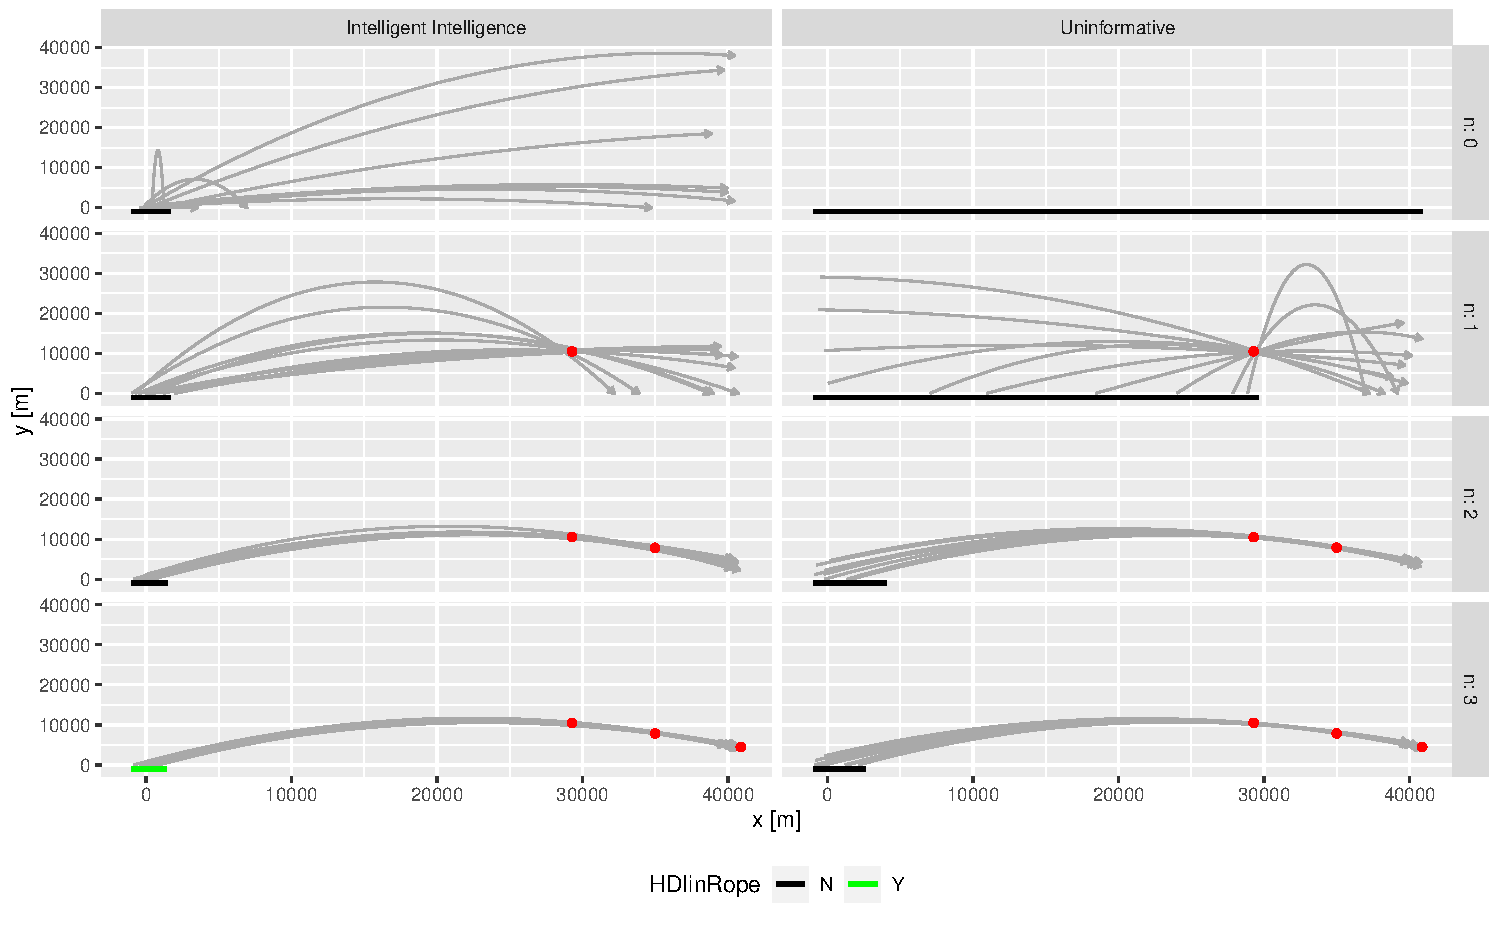
\includegraphics[width=1.0\textwidth]{bayesian_artillery_files/figure-latex/plot_full-1} \end{center}

Each grey line is a credible trajectory: we sample 10 quartets at random
from the posterior chain (actually the prior for n=0) and draw the
corresponding trajectory. This is a wonderful way to visualize what the
Bayesian procedure is, so to speak, ``thinking'' and ``believing''.

The red dots are the radar readings used to compute the posterior; it is
manifest that the credible trajectories pass ``near''\footnote{The
  smaller the radar \(\sigma_e\), the closest they pass near the
  readings (not shown here but easy to check)} them, as intuitively
expected.

The trajectories originate from the credible \(p0x\) positions;
underneath them the 95\% HDI\footnote{Highest Density Interval, again
  check (Kruschke \protect\hyperlink{ref-DBDA2E}{2015}, definition at
  page 28 and used all around the book)} of \(p0x\) is drawn, that can
be intuitively described as the region the contains the 95\% most
credible positions of the battery.

The HDI turns green when it is completely contained inside the ROPE, the
Region Of Practical Equivalence (Kruschke
\protect\hyperlink{ref-DBDA2E}{2015}, definition at page 336), that we
might describe as the sets of points \emph{practically} equivalent to
the true position of the battery. ``Equivalent'' is defined by the
\emph{practical} purpose of our analysis: in this case we will assume
that we plan to send a drone to confirm the position of the battery, and
since our drone can explore a space of 1500m from the starting point (in
both directions) before running out of power, the ROPE interval is
centered at the true position and 2x1500m wide, because any starting
point inside this ROPE will \emph{equivalently} allow us to find the
battery (one or another, we don't care). When the 95\% HDI is inside the
ROPE, to the best of our knowledge (prior + data) the drone will find
the battery with (at least) 95\% probability.

Why 95\% and not, say, 40\%? In a real scenario we would compare the
value gained by finding the battery with the cost of the drone mission,
and decide a threshold accordingly. A 95\% threshold is compatible with
a very high cost compared to the gain: we want to be almost absolutely
sure the the drone is not wasted. If the drone were inexpensive, we
might choose a very low threshold instead, maybe even 10\%.

\hypertarget{n-0-before-the-first-reading}{%
\subsection{n = 0: before the first
reading}\label{n-0-before-the-first-reading}}

Let's zoom in to the priors:

\begin{center}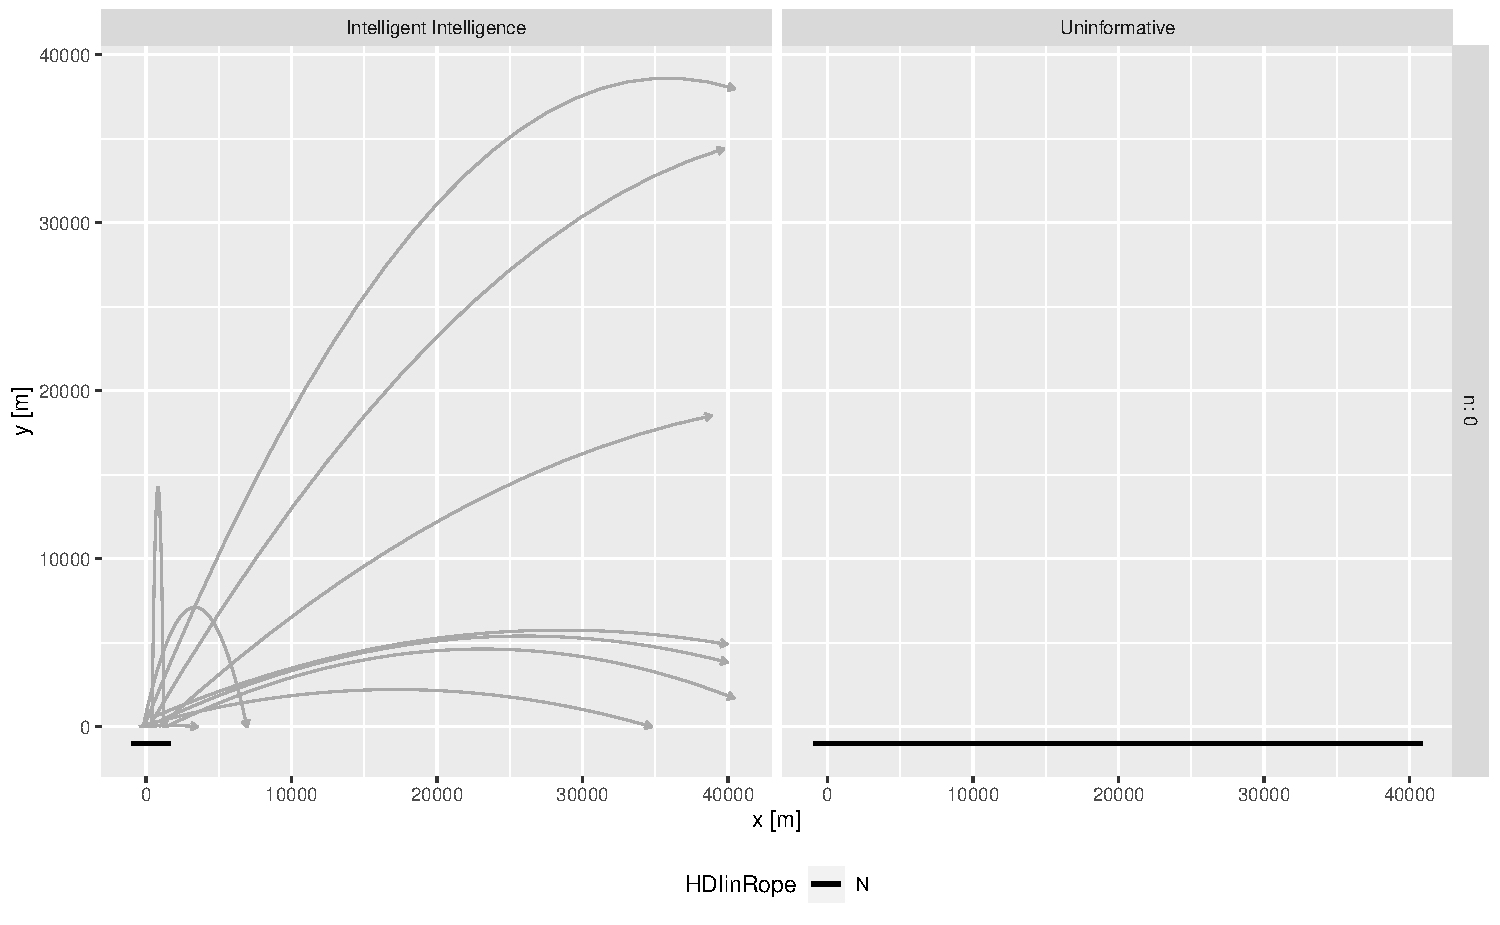
\includegraphics[width=1.0\textwidth]{bayesian_artillery_files/figure-latex/plot_0-1} \end{center}

The ``Intelligent Intelligence'' variant shoots credible projectiles
mostly from the HDI, but then the trajectories diverge quite wildly.
They do not diverge completely randomly, however, and exhibit quite a
strong regularity due to the other priors. In fact, the \(\theta\) prior
forces them all to point to the right (since the prior has exactly zero
density above \(\pi/2\)). And since \(v0\) is constrained below MACH3,
the kinetic energy is constrained as well, and that caps both the
maximun altitude and, indirectly, the maximum range in the x direction.
As a result, the credible trajectories do behave like a
weakly-coordinated flock.

The ``Uninformative'' variant shoots credible projectiles from random
points\footnote{the 95\% HDI extends well beyond the window shown - its
  width is actually a gigantic \ensuremath{4\times 10^{6}}m} in the
battlefield, and hence, even it shares the same other priors with the
former, it looks almost random. In fact the chances of passing inside
our narrow window over the battlefield are almost zero, and the right
window very frequently contains only a few trajectory fragments if any
at all (depending on the seeds set for JAGS/R pseudorandom generators).
Their credible trajectory shape is, however, the same as the other
variant.

\hypertarget{n-1-after-the-first-reading}{%
\subsection{n = 1: after the first
reading}\label{n-1-after-the-first-reading}}

\begin{center}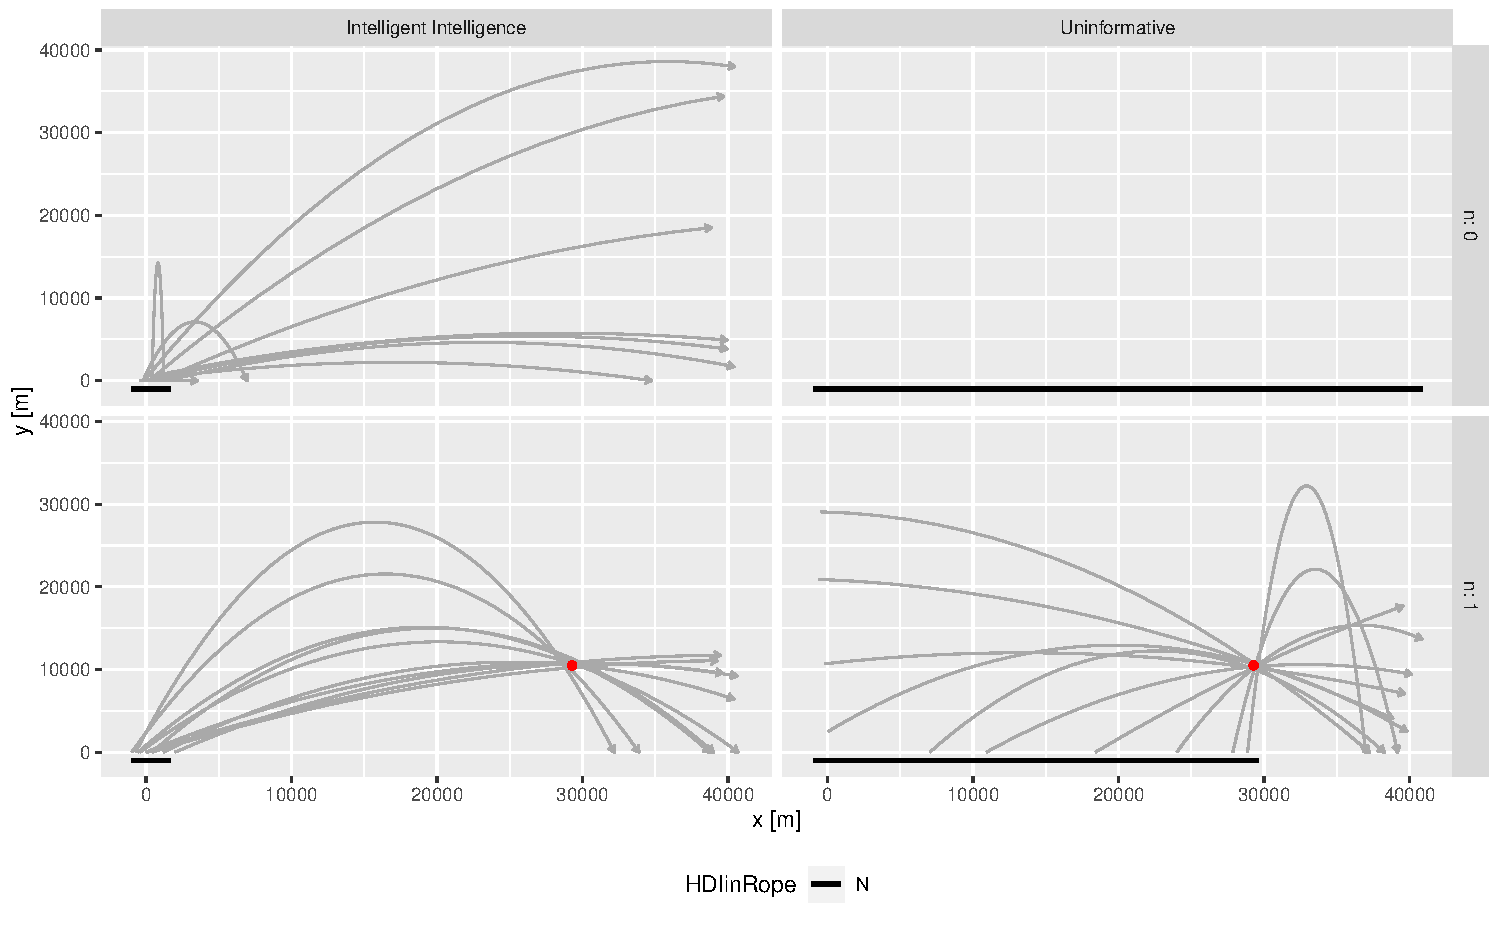
\includegraphics[width=1.0\textwidth]{bayesian_artillery_files/figure-latex/plot_1-1} \end{center}

As the first reading arrives, the credible trajectories cluster together
near the reading\footnote{because \(\sigma_e\) is relatively small
  compared to the trajectory}, since the Likelihood function value peaks
around it: the posterior peaks as well and, as a consequence, shrinks
everywhere else (the ``Reallocation of Credibility''\footnote{i.e.~check
  (Kruschke \protect\hyperlink{ref-DBDA2E}{2015}), especially figure 2.1
  on page 17, the best illustration I have ever seen} of Bayesian
Update).

It's instructive to describe how we could manually draw the approximate
credible trajectories using only elementary Statistics, Math and
Physics. Let's focus on the bottom left window. We could recall from
high-school that the trajectories are parabolic and hence with three
degrees of freedom (the three parameters in
\(y=\alpha_0 + \alpha_1x+\alpha_2x^2\)), and by varing the three
parameters we can position the parabola on the window wherever we want.
We choose a starting point inside the HDI and force the parabola to pass
there; this still leaves us two degrees of freedom. Then, we draw a
small circle centered on the reading with radius \(3*\sigma_e\): with
99\% probability the true trajectory passed through our circle, so we
choose another point there, and nail the parabola there as well.

We have still a degree of freedom, that allows the trajectory to vary
wildly (the projectile could for example get to the Moon\footnote{until
  now we have only factored-in the fact about the trajectory shape
  (parabolic), nothing has been said about the initial velocity,
  starting time, or travel time. It might as well travel to Alpha
  Centauri an back in 1 millisecond, since the model is classic and not
  relativistic, and hence the light-speed limit is not in effect.} and
back). Only by factoring in more prior knowledge we might get to a
family of trajectories roughly comparable to the Bayesian one; for
example we could constrain the maximum height of the parabola by
recalling that the initial kinetic energy is constrained by \(v_0\),
that is between MACH1 and MACH3 (doable but laborious).

Equivalently: choose a starting point inside the HDI, aim at the circle,
and fire. We can roughly factor in the prior on \(v0\) by choosing
different models of howitzers with different initial velocity, all
between MACH1 and MACH3.

In a way, the Bayesian algorithm does the same reasoning in this
scenario, but of course with much greater precision, sound statistical
background and less manual work from our part (or at least less boring).

As a final observation, note how this first reading has not altered that
much the HDI on the left window; the additional information has mainly
shrunken the credible trajectories (loosely speaking: by reducing their
degrees of freedom). The ``Uninformative'' scenario HDI is very
different instead: for example now it lays on the left of the reading,
thanks to the prior on \(\theta\), while the credible trajectories are
still quite free.

\hypertarget{n-2-after-the-second-reading}{%
\subsection{n = 2: after the second
reading}\label{n-2-after-the-second-reading}}

\begin{center}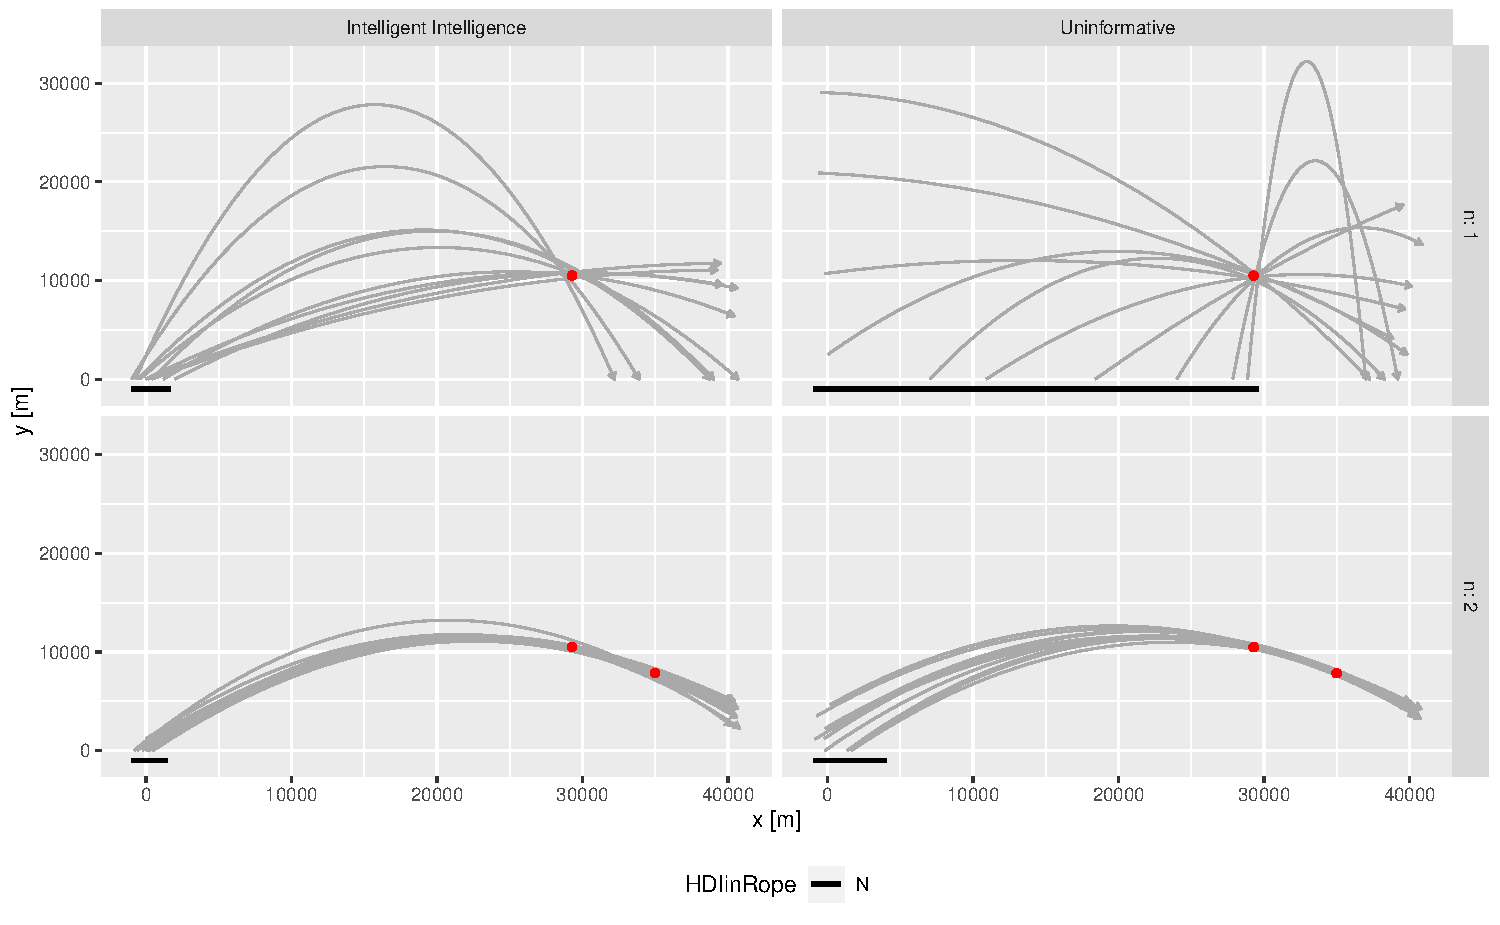
\includegraphics[width=1.0\textwidth]{bayesian_artillery_files/figure-latex/plot_2-1} \end{center}

Now with two readings, the credible trajectories gets clustered much
more around the true trajectory (that starts at x=0).

Using the manual methods, we would have now two points to nail the
parabola to (or to aim to), and a smaller room to start the trajectory,
and hence much less freedom for our projectile.

Again, the HDI shrinks much more for the ``Uninformative'' scenario on
the right.

\hypertarget{n-3-after-the-third-reading}{%
\subsection{n = 3: after the third
reading}\label{n-3-after-the-third-reading}}

\begin{center}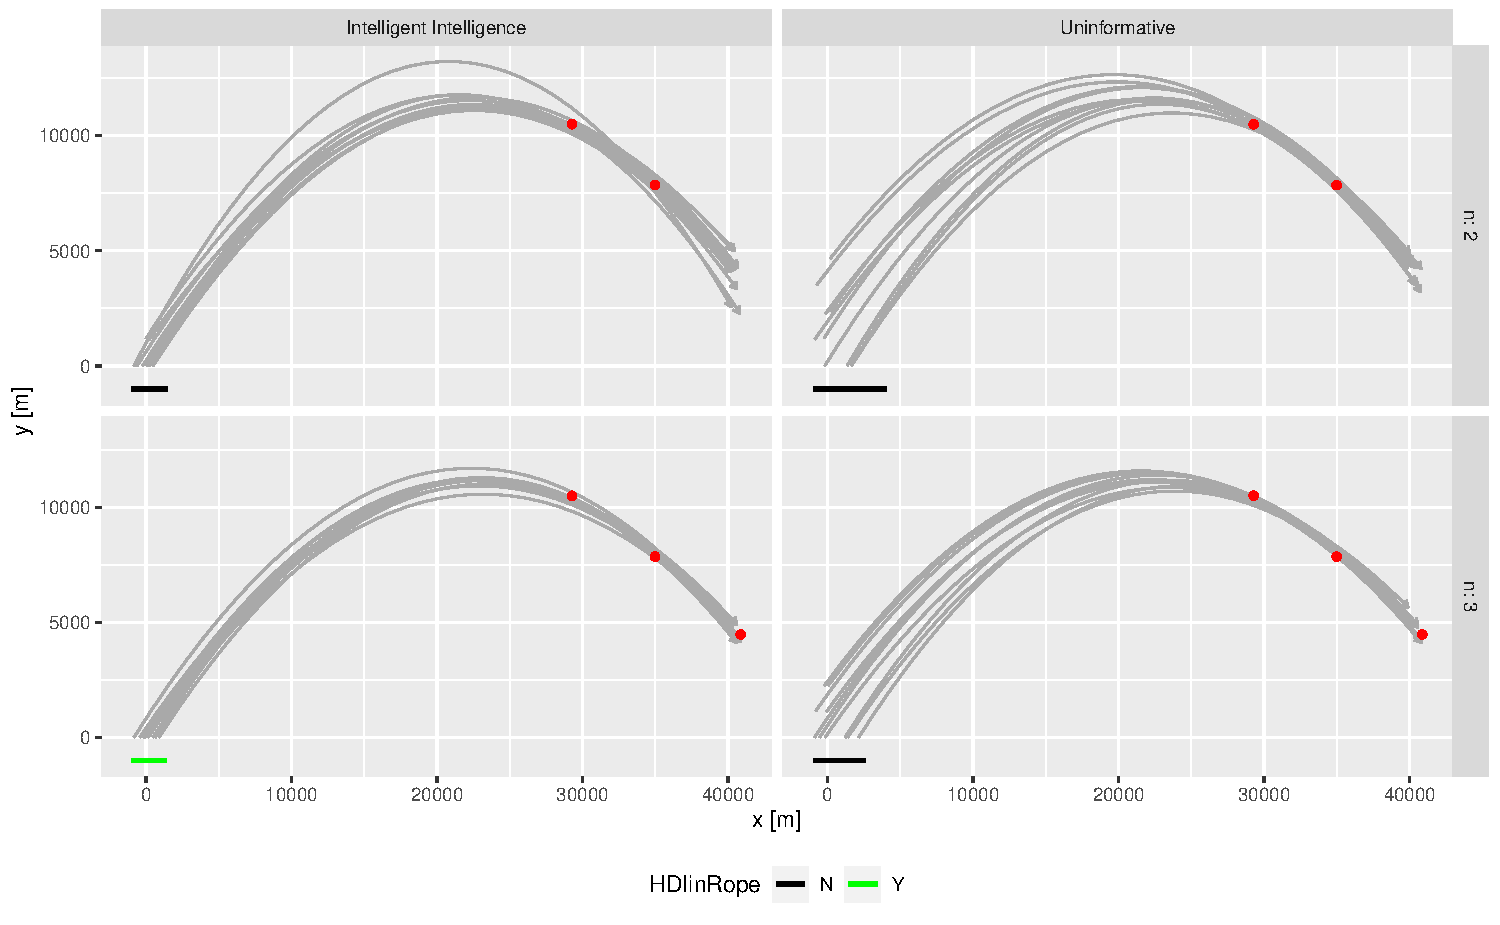
\includegraphics[width=1.0\textwidth]{bayesian_artillery_files/figure-latex/plot_3-1} \end{center}

At this point, if the three readings were noiseless, we could simply fit
the parabola to them and we would have inferred the exact position of
the battery, making the priors useless. But since \(\sigma_e\) is small
but not zero, there's still some room for the parabola to move around,
and hence opportunity for the priors to provide useful information by
influencing the prosterior; and in fact ``Intelligent Intelligence''
sets the green light to launch the drone, but that's not the case for
``Uninformative''.

\hypertarget{chains-convergence}{%
\section{Chains Convergence}\label{chains-convergence}}

We now breafly look at the converge diagnostics and accuracy of the
chains. We will look at \(p0x\), but I have checked all the other three
chain parameters as well and the results are the same, unless otherwise
noted.

Here are the four diagnostics diagrams suggested by (Kruschke
\protect\hyperlink{ref-DBDA2E}{2015}, especially chapter 7.5 on page
178) and implemented in his diagMCMC() function:

\begin{center}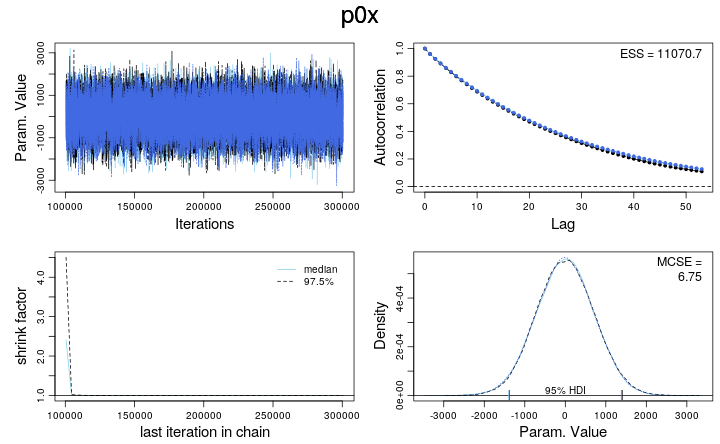
\includegraphics[width=1.0\textwidth]{bayesian_artillery_files/figure-latex/jags_convergence-1} \end{center}

We can see that, from the top left panel counterclockwise:

\begin{itemize}
\tightlist
\item
  the three chain jumps are qualitatively the same, with no orphans
\item
  the Gelman-Rubin statistic is well below 1.1
\item
  the three chains share the same estimated marginal density
\item
  the autocorrelation is high, but I have got enough samples to get over
  the minimum ESS (Effective Sample Size) of 10,000 that is
  empirically\footnote{from (Kruschke
    \protect\hyperlink{ref-DBDA2E}{2015}, 184): ``For reasonably
    accurate and stable estimates of the limits of the 95\% HDI, an ESS
    of 10,000 is recommended. This is merely a heuristic based on
    experience with practical applications''} needed to get good HDI
  accuracy and stability.
\end{itemize}

The other three parameters diagnostics (not shown) behave the same, but
the ESS is much lower (and this is not an issue since we are not
interested in their HDIs).

And of course - let's end with a souvenir photo of the longed-for
\(p0x\) posterior, showing the ROPE and the \(p0x\) true value:

\begin{center}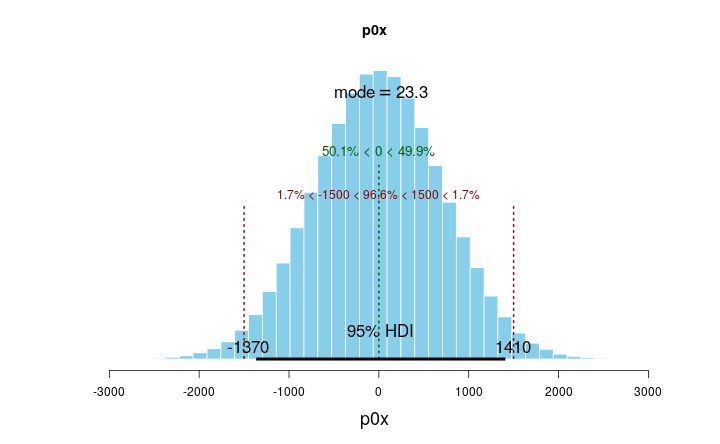
\includegraphics[width=1.0\textwidth]{bayesian_artillery_files/figure-latex/jags_posterior-1} \end{center}

We've found the battery!!

\hypertarget{next-steps}{%
\section{Next steps}\label{next-steps}}

Some ideas (and random thoughts) that I wrote down while I was working.

\hypertarget{air-friction-and-simulation}{%
\subsection{air friction and
simulation}\label{air-friction-and-simulation}}

The next most natural steps would be to consider air friction.

Closed-form solutions exist for special cases (e.g.~for air friction
force modulus equal to \(v^2(t)\)), and for those it is probably simple
to modify the likelihood accordingly. I would expect less precision in
the final \(p_0x\) estimation since now many more trajectories can
``pass near'' the radar readings\footnote{the models with air friction
  tends to produce trajectories that are more vertical near the end
  (since they admit a vertical asymptote), hence there are more credible
  trajectories compatible with \(\sigma_e\) - imagine a basketball hoop.
  Equivalently: if you integrate the model backwards in time, a small
  difference in the initial codition, compatible with \(\sigma_e\),
  makes a more different trajectory.}, that are located near the end of
the trajectories; but it would be fun to check out.

For a more realistic model, we would need to turn to simulation. The
real air friction dependency on \(v(t)\) is complex, it varies depending
on the speed of sound that in turn depends on air pressure and hence on
\(y(t)\), and it does not help that the projectile starts hypersonic and
(usually) ends subsonic, thus breaking the sound barrier at MACH1.

How to integrate a simulation in JAGS? I've investigated a bit and
discovered that JAGS could be extended not only by providing new
probability distributions, but also new functions. JAGS is written in
C++ and thus we could write the simulation in that language, incorporate
it in the JAGS source (it's open-source) and recompile; or maybe provide
the function as a shared library and relink.

\hypertarget{stan}{%
\subsection{Stan}\label{stan}}

Obviously, checking STAN would be very easy; I would expect similar
results, but maybe faster runtimes and less autocorrelation on the
posterior chains, since I suspect (by intuition only, I haven't checked)
that the posterior is constrained in the ``narrow valleys'' described in
(Kruschke \protect\hyperlink{ref-DBDA2E}{2015}, especially page 176). My
intuition should be verified of course.

\hypertarget{nimble}{%
\subsection{Nimble}\label{nimble}}

It would be very interesting to explore the Nimble tool
(\url{https://r-nimble.org/}), that extends the BUGS language (the
language of the JAGS models) to allow for easy integration of new
functions, written in simil-R, and compiles them in C++ before running.
On paper, it has the potential for being a fantastic toolset, worth
investing time into.

The simple frictionless model that we have discussed looks like a good
testcase to compare Nimble with JAGS (and maybe STAN), before turning to
simulation with air friction where it should show its full potential.

Document version: 2020/05/18

\hypertarget{references}{%
\section{References}\label{references}}

Gihub repository:
(\url{https://github.com/alberto-dellera/bayesian_artillery})

\hypertarget{refs}{}
\leavevmode\hypertarget{ref-DBDA2E}{}%
Kruschke, John K. 2015. \emph{Doing Bayesian Data Analysis: A Tutorial
with R, Jags, and Stan}. 2nd ed. Academic Press / Elsevier.
\url{https://sites.google.com/site/doingbayesiandataanalysis}.

\leavevmode\hypertarget{ref-JAGSmanual}{}%
Plummer, Martyn. 2017. \emph{JAGS Manuals}.
\url{https://sourceforge.net/projects/mcmc-jags/files/Manuals/4.x/}.

\end{document}
